
    \documentclass{article}

    %  Русский язык

    \usepackage[T2A]{fontenc}			% кодировка
    \usepackage[utf8]{inputenc}			% кодировка исходного текста
    \usepackage[english,russian]{babel}	% локализация и переносы
    \usepackage{unicode-math}

    % Рисунки
    \usepackage{graphicx, float}
    \usepackage{wrapfig}


    \title{Wild wild west derivative counter}
    \author{Dodo}
    \date{November 2022}


    \begin{document}
    \maketitle
    
        Welcome to derivative calculator fella, let's have a look at ya. God, what da hell is dis shit, fella?
        Ok, ok, let's calculate this bullshit.

        \begin{center}\begin{figure}[H] 
\includegraphics[scale=0.6]{funny_pics/cowboy.jpg} \end{figure}\end{center}
        \begin{center}
        $\clubsuit$~$\clubsuit$~$\clubsuit$
        \end{center}

    \begin{figure}[H] 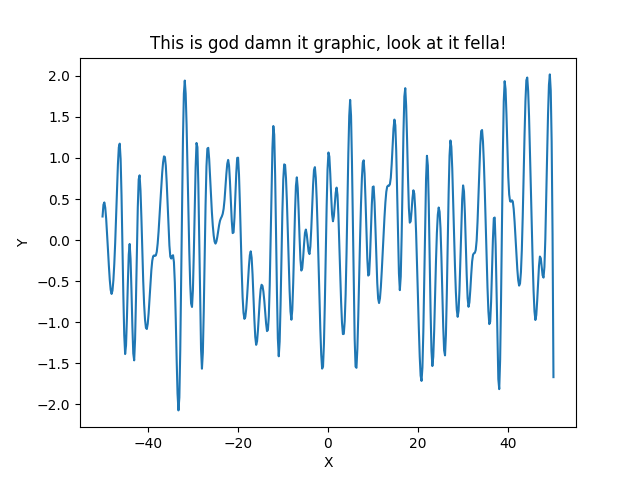
\includegraphics[scale=0.6]{function_graph.png} \end{figure}Alright fella, let's look wat we got:

\begin{equation}
{{sin({X})}+{\frac{({cos({{X}+{5}})})}{({ln({{5}+{{2}\cdot{X}}})})}}}
\end{equation}
\begin{center} $\clubsuit$~$\clubsuit$~$\clubsuit$ \end{center}\begin{figure}[H] 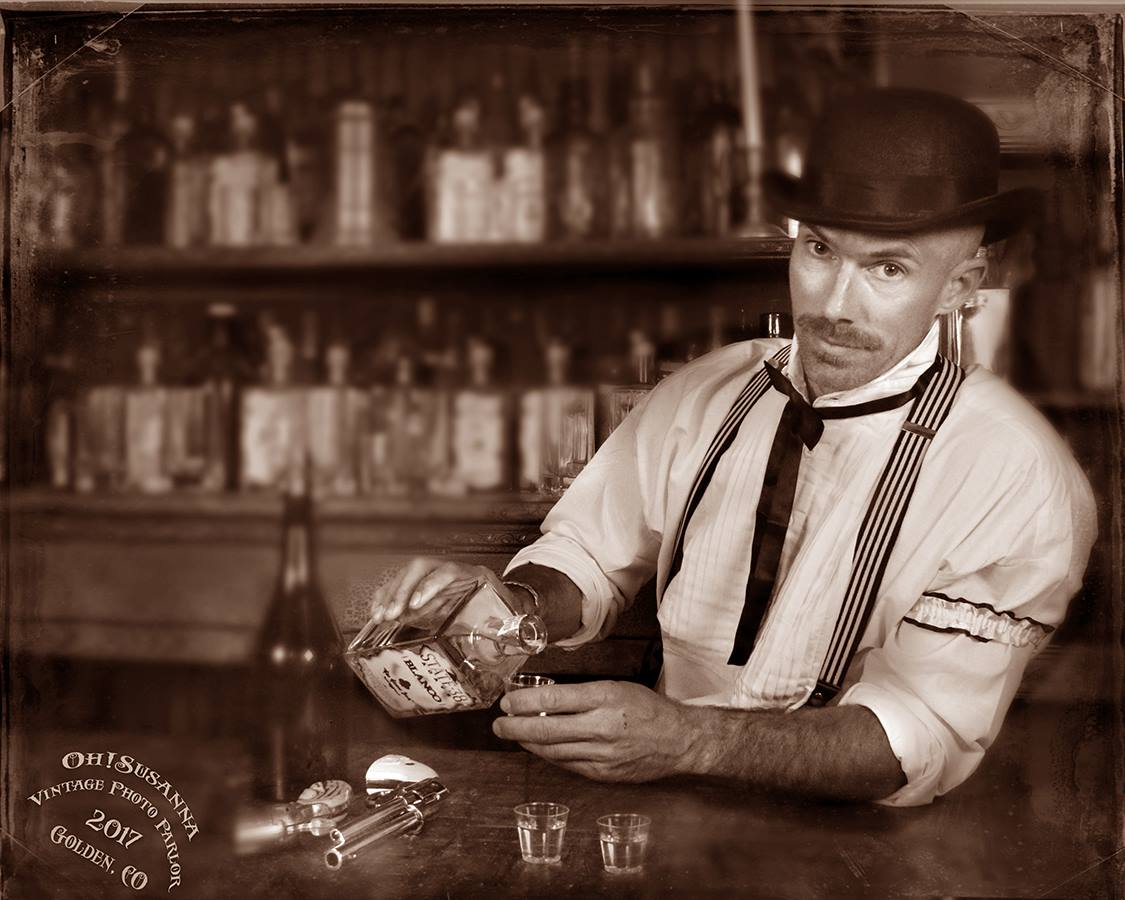
\includegraphics[scale=0.3]{funny_pics/bartender.jpg} \end{figure} With the power of gods, let's write the following: 
\begin{equation}
{{sin({X})}+{\frac{({cos({{X}+{5}})})}{({ln({{5}+{{2}\cdot{X}}})})}}}
\end{equation}
\begin{center} $\clubsuit$~$\clubsuit$~$\clubsuit$ \end{center}\begin{figure}[H] 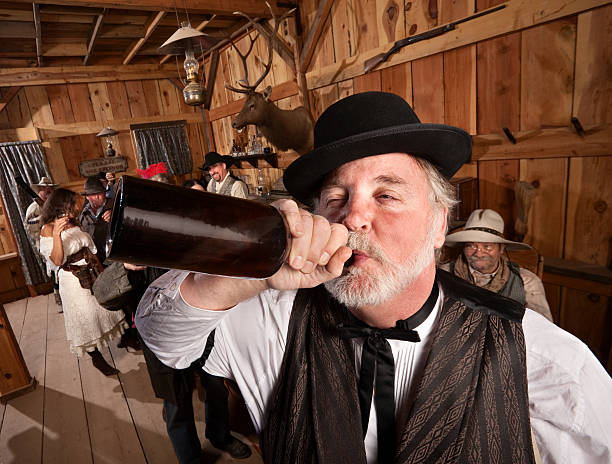
\includegraphics[scale=1.4]{funny_pics/drunk_cowboy.jpg} \end{figure} I smacked a damn big cockroach yesterday fella, this was left on my shoe: 
\begin{equation}
{\frac{({cos({{X}+{5}})})}{({ln({{5}+{{2}\cdot{X}}})})}}
\end{equation}
\begin{center} $\clubsuit$~$\clubsuit$~$\clubsuit$ \end{center}\begin{figure}[H] 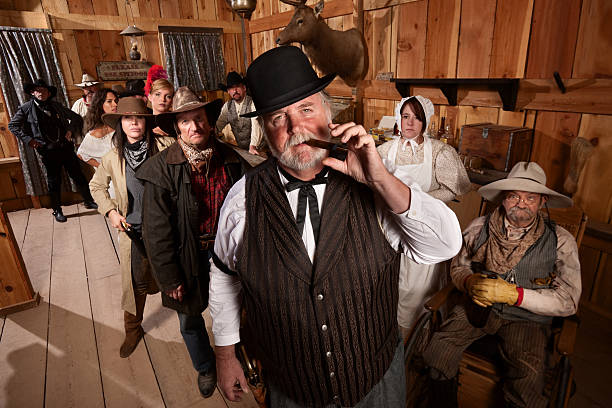
\includegraphics[scale=1.4]{funny_pics/funny_bartender.jpg} \end{figure} Don't distract fella, I don't know how to count
\begin{equation}
{ln({{5}+{{2}\cdot{X}}})}
\end{equation}
\begin{center} $\clubsuit$~$\clubsuit$~$\clubsuit$ \end{center}\begin{figure}[H] 
\includegraphics[scale=0.3]{funny_pics/cowboy_cat.jpg} \end{figure}Oh come on, my wife is pregnant 12th time in a row.
\begin{equation}
{{5}+{{2}\cdot{X}}}
\end{equation}
\begin{center} $\clubsuit$~$\clubsuit$~$\clubsuit$ \end{center}\begin{figure}[H] 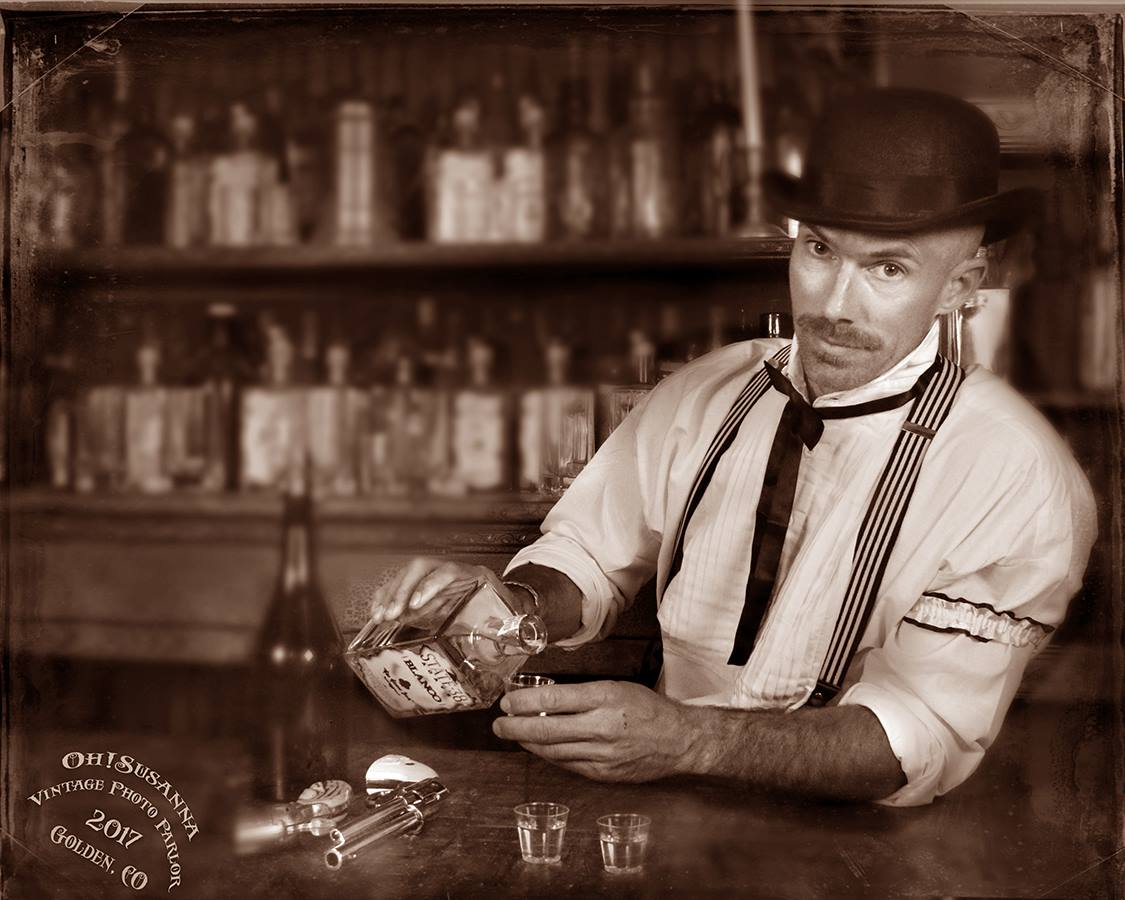
\includegraphics[scale=0.3]{funny_pics/bartender.jpg} \end{figure}Can you understand it by yourself, i must go get some beer, fella:
\begin{equation}
{{2}\cdot{X}}
\end{equation}
\begin{center} $\clubsuit$~$\clubsuit$~$\clubsuit$ \end{center}...
\begin{equation}
{cos({{X}+{5}})}
\end{equation}
\begin{center} $\clubsuit$~$\clubsuit$~$\clubsuit$ \end{center}\begin{figure}[H] 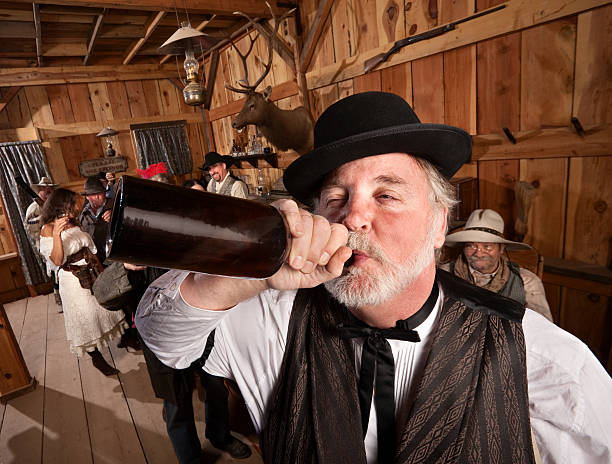
\includegraphics[scale=1.4]{funny_pics/drunk_cowboy.jpg} \end{figure}Thanks man
\begin{equation}
{{X}+{5}}
\end{equation}
\begin{center} $\clubsuit$~$\clubsuit$~$\clubsuit$ \end{center}I don't fucking know how this expression was calculated, fella, i am a cowboy
\begin{equation}
{sin({X})}
\end{equation}
\begin{center} $\clubsuit$~$\clubsuit$~$\clubsuit$ \end{center}Here is whach you got, fella. Now let's drink some whiskey and shoot niggers.\begin{figure}[H] 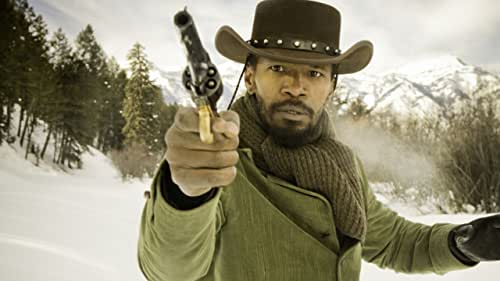
\includegraphics[scale=0.6]{funny_pics/slave.jpg} \end{figure}
\begin{equation}
{{({cos({X})})\cdot({1})}+{\frac{({{({({({-1})\cdot({sin({{X}+{5}})})})\cdot({1})})\cdot({ln({{5}+{{2}\cdot{X}}})})}-{({cos({{X}+{5}})})\cdot({({\frac{({1})}{({{5}+{{2}\cdot{X}}})}})\cdot({2})})}})}{({({ln({{5}+{{2}\cdot{X}}})})\cdot({ln({{5}+{{2}\cdot{X}}})})})}}}
\end{equation}
\begin{center} $\clubsuit$~$\clubsuit$~$\clubsuit$ \end{center}Alright fella, let's make this shit called <Macloren>,there will be only 3 steps, cause i don't know how to count more.Basicly the main formula will look like that
 \[ f(x) = f(0) + \frac{f^{(1)}(0)}{1!}\cdot X + \frac{f^{(2)}(0)}{2!}\cdot X + \frac{f^{(3)}(0)}{3!}\cdot X + \text{...}\]
\[ f^{(0)}(0) = 0.176249\]\[ f^{(1)}(0) = 1.55201\]\[ f^{(2)}(0) = -0.433114\]\[ f^{(3)}(0) = -1.12227\]
        The solution is pretty simple and you definetely can do it \textbf{yourself}
        \end{document}
    